\documentclass[conference]{IEEEtran}
\usepackage[T1]{fontenc}
\usepackage{graphicx}
\usepackage{booktabs}
\usepackage{array}
\newcolumntype{L}[1]{>{\raggedright\arraybackslash}p{#1}}
\usepackage{amssymb}
\usepackage{stfloats}
\usepackage{microtype}
\usepackage{url}
\usepackage[hidelinks]{hyperref}

\newcommand{\K}{$K$}
\newcommand{\x}{$\times$}
\newcommand{\pick}{$^\star$}
\newcommand{\pickf}{$^{\star-}$}
\newcommand{\topk}{$^\dagger$}
\newcommand{\cfg}[1]{\texttt{#1}}
\setlength{\textfloatsep}{9pt plus 2pt minus 2pt}
\setlength{\dbltextfloatsep}{9pt plus 2pt minus 2pt}

\begin{document}

\title{Memory-Aware Agent Edge Serving:\\
\large Reclaiming Idle KV Cache at Tool-Call Boundaries}

\author{\IEEEauthorblockN{Jiawei Liu, Kaiqi Han, Tianyu Xu, You Chen, Yufan Shi}
\IEEEauthorblockA{CSE 291A, Fall 2026}}

\maketitle

\begin{abstract}
LLM agents alternate model calls with tool calls and keep their KV cache while they wait; on a small
GPU this idle KV, not compute, limits how many agents can run. We serve HotpotQA ReAct agents with
Qwen2.5-7B on an unmodified \texttt{llama-server} under a fixed KV pool and reclaim idle KV from the
client with three levers: an exact ledger and gate that let the pool be committed without overflow; a
lifecycle that offloads, drops to the shared prefix or erases idle agents' KV under pressure; and
TRIM, which rewrites each tool observation the agent has already read to its useful sentences. At
two tight operating points, the full manager raises goodput over a tuned fixed concurrency by
26--34\% on dev and 17--41\% on a held-out test split (14--22\% on dev without its host-RAM tier),
with equivalent answer quality. A 2\x2 decomposition attributes most of this to the gate, which lets
a higher concurrency run safely, and 10--16\% to the lifecycle; peak-projection admission adds
nothing. TRIM cuts the KV held during tool calls by 25--28\% and raises F1 by 0.03--0.05; at
16k\,\x4 it lets fixed concurrency run 50\% more agents (+46--53\%), the best result there, while at
8k\,\x1 the manager stays ahead. The levers draw on the same idle KV and do not add up: with
admission tuned for untrimmed agents, the manager spends TRIM's savings on extra agents and recompute.
\end{abstract}

\section{Introduction}

An agent's context grows with every tool result, and between model calls its KV cache sits idle
while a search or a program runs. Serving engines see requests, not agents: they either keep the
idle KV, which caps concurrency, or discard it and recompute the whole context when the agent
returns. Measuring HotpotQA~\cite{hotpotqa} ReAct agents~\cite{react} on an A10G with Qwen2.5-7B
Q4\_K\_M~\cite{qwen} and \texttt{llama-server}~\cite{llamacpp}, we found that contexts grow 2--4\x{}
within a task, so a fixed concurrency \K{} must reserve the pool for all \K{} agents' simultaneous
peaks; that over-committing the pool fails every in-flight request at once; that in tight pools
agents waiting on tools hold 36--44\% of the KV; and that only about 13\% of the observation text an
agent carries is supporting facts or page titles. The question is what to do with an idle agent's
KV: keep it, move it, throw it away, or keep only part of it.

Our answer, measured at two tight operating points: \emph{keep it, but count it exactly}. An exact
ledger lets the pool be committed safely, and that alone gives most of the gain (+17--25\% over a
tuned fixed \K). \emph{Move or throw it away per agent under pressure} rather than letting the server
purge it: +10--16\%, consistent but significant in one of four tests; llama.cpp's own host-RAM cache
trails the manager by 11--34\%. \emph{Keep only the useful part}: trimming observations the agent has
read cuts tool-wait KV by a quarter, improves answers, and where trimmed agents fit a higher
concurrency it is the largest single gain we measured. The levers reclaim the same idle KV, so
combining them needs an admission policy that knows about all of them.

Contributions: \emph{(i)} a client-side KV manager on an unmodified edge server, using only
\texttt{llama-server}'s HTTP controls (Sec.~\ref{sec:design}); \emph{(ii)} TRIM, sentence-level
selective KV at tool-call boundaries, with HotpotQA's supporting facts as an oracle
(Sec.~\ref{sec:trim}); \emph{(iii)} an evaluation with tuning and decision rules fixed in advance
(deviations in Sec.~\ref{sec:disc}): a comparison at four operating points, a held-out test split, a
2\x2 decomposition at both tight points, and a study of how TRIM composes with the manager, including a
negative result and the rule that fixes it (Sec.~\ref{sec:results}).

\emph{Related work.} PagedAttention~\cite{vllm} removes fragmentation and lets requests share prefix
blocks; SGLang~\cite{sglang} reuses prefixes across requests. Both manage KV per request.
InferCept~\cite{infercept} is closest: for requests paused by tool calls inside vLLM it chooses
among preserving, discarding and swapping the KV to minimize waste. We make that choice per agent
from outside an unmodified edge server, and add a fourth option, keeping part of the context. Prompt
compression~\cite{llmlingua} and KV eviction~\cite{h2o} shorten contexts by token importance; TRIM
works at sentence level on tool output the agent has already read, at a point where it is known to
have been consumed.

\section{Design}\label{sec:design}

The design uses only controls \texttt{llama-server} b11960 already has: \texttt{/completion} pinned
to a slot (\texttt{id\_slot}) with prefix reuse, \texttt{/tokenize}, \texttt{/slots}, and slot save,
restore and erase. Table~\ref{tab:runtime} lists what probing them taught us; llama.cpp and the agent
are unchanged.

\begin{table}[t]
  \caption{Runtime Facts Behind the Design (b11960, A10G)}
  \label{tab:runtime}
  \centering
  \scriptsize
  \setlength{\tabcolsep}{2.5pt}
  \begin{tabular}{@{}L{0.13\columnwidth}L{0.55\columnwidth}L{0.28\columnwidth}@{}}
    \toprule
    Probe & Observation & Consequence \\
    \midrule
    Pool full & idle slots purged in id order, then all processing slots fail & active KV is a
      hard limit \\
    Idle slots & 4 decoders: 293 $\rightarrow$ 203 tok/s with 16 idle \x{} 3k; attention spans up
      to the top occupied cell & idle KV costs compute only if it holds top cells \\
    Drop to prefix & prefix ids with $n_\mathrm{predict}=0$: 19.6\,ms; revisit reuses all 1,421 &
      keep the prefix; TRIM uses the same path \\
    Busy slot & save is deferred until the stream ends & ops on idle slots only \\
    Save, restore & 59.0 + 30.0\,\textmu s/tok in the probe (online fit under load: 83--245) vs.\
      281\,\textmu s/tok re-prefill & offload can beat re-prefill for long tails \\
    Host cache & \texttt{-{}-cache-ram} saves and clears idle slots at each launch; pinned slots
      never reload & B2 runs unpinned \\
    \bottomrule
  \end{tabular}
\end{table}

\subsection{Accounting and the Gate}\label{sec:gate}
Slot $k$'s resident count after a response is $s_k=\mathit{prompt\_n}+\mathit{cache\_n}+
\mathit{predicted\_n}-1$ (the last sampled token has no KV yet). Its charge $u_k$ is $s_k$ when idle,
0 when offloaded, and $\max(s_k,f)$ while a request with $f=\mathrm{tok}(P)+n_\mathrm{predict}$ runs,
since llama.cpp drops a slot's old tail only when the new prompt enters a batch. A request for slot
$k$ dispatches only if $\sum_j u_j-u_k+\max(s_k,f)\le c-m$ ($c$: pool size, $m=128$ cells of margin).
With exact \texttt{/tokenize} (it matched the server on 550/550 prompts), this \emph{full gate}
excludes overflows and server purges. Keeping every idle slot under it would deadlock, since the agents
filling the pool are the ones waiting for room, so configurations that leave idle KV to llama.cpp use
an \emph{active gate} that charges in-flight requests only and lets the server purge idle slots
(appendix: a bug in its first version).

\subsection{Admission}
A task is admitted while all agents' projected peaks (current size plus the 0.9-quantile of remaining
growth, fitted offline per workload profile) fit $(1+\omega)(c-m)$, up to $K_\mathrm{max}=8$ at delay
scale \x1 or 16 at \x4 (Sec.~\ref{sec:setup}).

\subsection{Lifecycle}
When the request at the head of the gate queue lacks room, idle agents are given up one at a time:
finished tasks first, then the agent expected to return last. An online cost model picks
\emph{offload} to host RAM (a tier of $h\cdot c$ tokens, $h=1$), \emph{drop} to the shared ReAct
prefix (1,421 or 1,633 tokens, one per profile), or \emph{erase}. Returning agents reclaim memory at
once; a new task takes idle KV only after a pressure-gated ski-rental TTL, so nothing is given up
without pressure.

\subsection{TRIM: Keeping Only the Useful Part}\label{sec:trim}
The ReAct prompt is append-only, so observation $n$ is read at full length exactly once, by the
request that writes Thought/Action $n{+}1$; after that, the agent's own Thought restates what it took
from it. Right after that request, before the tool call starts, TRIM sends one prefill-only request
($n_\mathrm{predict}=1$) whose prompt replaces observation $n$ with the sentences a selector keeps
(page titles and tool messages are always kept; a run of dropped sentences becomes ``\ldots''). The
server reuses the common prefix and re-prefills only the shortened tail (about 130 tokens), so the slot
holds the compacted context during the tool wait and the next request is append-only again. It is the
drop-to-prefix path with a different target. Selectors: \cfg{oracle} keeps HotpotQA's supporting
facts, an upper bound on what selection can keep for free; \cfg{relevance:$r$} keeps the $r$
sentences per observation with the highest IDF-weighted word overlap with the question;
\cfg{referenced} keeps sentences sharing a salient word with the agent's next Thought/Action;
\cfg{drop} keeps titles only.

\subsection{Composition at the Gate}\label{sec:sf}
A compaction is a request with $f\le s_k$, charged $\max(s_k,f)=s_k$: it needs no new memory. Queued
like any other request, though, it waits behind the gate's head, and a slot whose agent waits there is
an eligible victim, so the manager may give up KV seconds before it would have shrunk. The
\emph{shrink-fast} rule dispatches a request that only shrinks its owner's resident slot at once and
never takes such a slot as a victim. Its charge equals the slot's current one, so it delays no other
request, and append-only requests ($f>s_k$) are unaffected. We added this rule after the first
composed runs; Sec.~\ref{sec:compose} reports both.

\section{Setup}\label{sec:setup}

\emph{Runtime and workload.} \texttt{llama-server} b11960 on an A10G serves Qwen2.5-7B-Instruct
Q4\_K\_M with f16 KV in one unified pool of $c$ cells (\texttt{-c}, \texttt{-{}-kv-unified}).
Agents answer HotpotQA questions over a 66,581-page offline corpus in a mix of 70\%
\texttt{react\_long} (10 paragraphs per search) and 30\% \texttt{react\_short}. All tasks are released
at $t=0$; tool delays are lognormal (median 0.8\,s), seeded, and scaled by \x1 or \x4.

\emph{Splits and operating points.} Knobs are tuned on 200 questions of a \emph{perf} split, one run
per knob; results are fresh runs on 200 \emph{dev} questions (3 reps) and, for the headline claim, 500
held-out \emph{test} questions (2 reps, every knob frozen); the splits are disjoint. An operating
point such as 16k\,\x4 names the pool $c$ and the delay scale: 16k\,\x4 and 8k\,\x1 are the tight
points, 16k\,\x1 and 32k\,\x4 were pre-registered as low-benefit, and 131k\,\x1 is a no-pressure check.

\emph{Configurations} (Table~\ref{tab:cfg}). Fixed-\K{} configurations use \K{} as their knob, KV
admission uses $\omega$. Ablations change one rule of \cfg{ours} at 16k\,\x4 (e.g.\ \cfg{act\_erase}
never offloads or drops, \cfg{act\_offload} always offloads, \cfg{always\_off} offloads at every tool
start).

\begin{table}[t]
  \caption{Configurations}
  \label{tab:cfg}
  \centering
  \scriptsize
  \setlength{\tabcolsep}{3pt}
  \begin{tabular}{@{}lllll@{}}
    \toprule
    Config & Concurrency & Gate & Idle KV & Host RAM \\
    \midrule
    \cfg{B1} & fixed \K, pinned & none & llama.cpp purge & -- \\
    \cfg{B2} & fixed \K, unpinned & none & llama.cpp host cache & $h\cdot c$ \\
    \cfg{gated\_k} & fixed \K & active & llama.cpp purge & -- \\
    \cfg{adm\_retain} & KV admission & active & llama.cpp purge & -- \\
    \cfg{managed\_k} & fixed \K & full & our lifecycle & $h\cdot c$ \\
    \cfg{ours} & KV admission & full & our lifecycle & $h\cdot c$ \\
    \cfg{ours\_h0} & KV admission & full & lifecycle, no offload & -- \\
    \cfg{B1+X} & as \cfg{B1}, \K{} retuned & none & kept, trimmed & -- \\
    \cfg{ours+X} & as \cfg{ours} & full & lifecycle, trimmed & $h\cdot c$ \\
    \bottomrule
  \end{tabular}\\[2pt]
  \parbox{\columnwidth}{\raggedright\scriptsize Idle KV: what happens to it under pressure (``llama.cpp
  purge'': kept until the server purges it). X: TRIM with \cfg{oracle} or \cfg{relevance:2} (\cfg{rel2}).}
\end{table}

\emph{Tuning.} For each configuration and point, the chosen knob has the highest goodput among those
completing ${\ge}95\%$ of tasks (\pick; \pickf{} when none does, the highest completion); B1 is also
reported at its best-goodput \K{} (\topk). TRIM was set up by the same rules before its runs: the
selector is chosen on perf at ample memory (64k\,\x1, B1 $K{=}8$, 2 reps) as the realistic selector
(\cfg{relevance:2}, \cfg{relevance:3} or \cfg{referenced}) with the smallest mean peak context among
those whose mean F1 is at most 0.03 below no trimming; the admission priors are refit on those runs;
B1's \K{} is retuned per selector (appendix). \cfg{ours} keeps the $\omega$ tuned without TRIM
($\omega{=}1$ at both tight points).

\emph{Metrics.} Goodput is EM-correct tasks per minute over the whole run, failures counted wrong;
completion is the share answered. A difference is \emph{supported} (S) only if Welch's $p<0.05$ on
per-run goodput \emph{and} the bootstrap 95\% CI of the difference in steady goodput (the 10--90\%
completion window) excludes 0, else \emph{not established} (n.e.). Quality: paired per-question F1
TOST over questions answered in every run on both sides, margin $\pm0.05$ (dev) or $\pm0.03$ (test).

\begin{table*}[!t]
  \caption{The Manager vs.\ Fixed Concurrency on the Dev Split (200 Tasks per Run; Mean over Reps, Min--Max)}
  \label{tab:main}
  \centering
  \scriptsize
  \setlength{\tabcolsep}{2.7pt}
  \renewcommand{\arraystretch}{0.9}
  \begin{tabular}{@{}lllrcrcrrrrrcc@{}}
    \toprule
    Point & Config & Knob & Done & Goodput & Agents & Give-ups & Recomp. & Op & Purges / &
      \multicolumn{4}{c}{\cfg{ours} vs.\ this row} \\
    \cmidrule(l){11-14}
     (reps) & & & (\%) & (correct/min) & & total (off/drop/erase) & (tok/task) & (\%) & overflows
      & $\Delta$ (\%) & $p$ & Steady 95\% CI & Verdict \\
    \midrule
    16k\,\x4 & \cfg{B1}\pick & $K{=}4$ & 98.8 & 10.97 (10.86--11.11) & 3.9 & -- & 31 & -- & 3 / 1 &
      +33.6 & 0.01 & [+2.35, +5.75] & S \\
    (3) & \cfg{B1}\topk & $K{=}6$ & 88.5 & 13.95 (13.19--15.22) & 5.9 & -- & 187 & -- & 25 / 4 &
      +5.0 & 0.40 & [$-$0.93, +3.06] & n.e. \\
     & \cfg{B2} & $K{=}6$, 896\,MiB & 85.3 & 13.23 (12.47--14.62) & 5.9 & -- & 626 & -- & 0 / 5 &
      +10.8 & 0.17 & [$-$0.34, +3.89] & n.e. \\
     & \cfg{ours} & $\omega{=}1$ & \textbf{100.0} & \textbf{14.66} (13.98--15.11) & 6.8 &
      208 (89/118/45) & 472 & 10.5 & 0 / 0 & & & & \\
    \midrule
    8k\,\x1 & \cfg{B1}\pickf & $K{=}2$ & 92.0 & 12.92 (12.65--13.34) & 2.0 & -- & 8 & -- & 3 / 8 &
      +26.2 & $<$0.001 & [+1.37, +5.16] & S \\
    (3) & \cfg{B1}\topk & $K{=}3$ & 64.2 & 13.91 (13.30--14.71) & 3.0 & -- & 71 & -- & 28 / 24 &
      +17.3 & 0.02 & [+0.52, +4.74] & S \\
     & \cfg{B2} & $K{=}2$, 448\,MiB & 91.3 & 12.21 (11.99--12.51) & 2.0 & -- & 244 & -- & 0 / 9 &
      +33.6 & $<$0.001 & [+2.05, +5.66] & S \\
     & \cfg{ours} & $\omega{=}1$ & \textbf{98.8} & \textbf{16.31} (16.09--16.43) & 3.2 & 179 (97/82/57) &
      538 & 8.9 & 0 / 0 & & & & \\
    \midrule
    16k\,\x1 & \cfg{B1}\pick & $K{=}3$ & 100.0 & 17.38 (16.63--18.33) & 3.0 & -- & 6 & -- & 1 / 0 &
      +28.9 & 0.004 & [+1.74, +7.25] & S \\
    (3) & \cfg{B1} & $K{=}4$ & 97.3 & 22.05 (21.81--22.49) & 4.0 & -- & 6 & -- & 2 / 1 &
      +1.6 & 0.32 & [$-$2.95, +2.69] & n.e. \\
     & \cfg{B1}\topk & $K{=}5$ & 92.5 & 23.86 (23.52--24.27) & 5.0 & -- & 20 & -- &
      5 / 3 & $-$6.1 & 0.01 & [$-$6.52, $-$0.18] & S \\
     & \cfg{B2} & $K{=}4$, 896\,MiB & 98.0 & 17.78 (17.22--18.43) & 4.0 & -- & 324 & -- & 0 / 1 &
      +26.1 & $<$0.001 & [+1.77, +6.90] & S \\
     & \cfg{ours} & $\omega{=}0.5$ & \textbf{100.0} & \textbf{22.41} (22.03--22.82) & 5.1 &
      41 (23/18/11) & 96 & 5.4 & 0 / 0 & & & & \\
    \midrule
    32k\,\x4 & \cfg{B1}\pick\topk & $K{=}8$ & 100.0 & 18.54 (18.07--19.13) & 7.8 & -- & 10 & -- & 1 / 0 &
      +8.7 & 0.03 & [$-$1.32, +3.59] & n.e. \\
    (3; B2: 2) & \cfg{B2} & $K{=}8$, 1,792\,MiB & 100.0 & 16.10 (15.71--16.49) & 7.8 & -- & 668 & -- & 0 / 0
      & +25.2 & 0.01 & [+1.24, +6.47] & S \\
     & \cfg{ours} & $\omega{=}0.5$ & \textbf{100.0} & \textbf{20.16} (19.49--20.76) & 10.4 &
      15 (11/4/3) & 21 & 2.7 & 0 / 0 & & & & \\
    \bottomrule
  \end{tabular}\\[2pt]
  \parbox{\textwidth}{\raggedright\scriptsize \pick{} perf pick; \pickf{} fallback (no \K{} reaches 95\%);
  \topk{} perf top-goodput \K. Failures: baselines' are context overflows; \cfg{ours} loses 2.3
  \texttt{kv\_infeasible} tasks/run at 8k\,\x1 (a context that cannot fit the pool). Agents: time-mean in
  flight. Give-ups per run: idle periods in which an agent's KV was given up (one event even if a drop
  is followed by an erase), by action. Recomp.: re-prefilled tokens/task, from the traces. Op: slot-op
  time/makespan. --: not applicable, or (B2) done inside llama.cpp and invisible to the client.}
\end{table*}

\section{Results}\label{sec:results}

\subsection{The Manager vs.\ Fixed Concurrency}\label{sec:main}
Against \cfg{B1}\pick{} (Table~\ref{tab:main}), \cfg{ours} completes as many or more tasks at every
point, and its gain is supported at both tight points: +33.6\% at 16k\,\x4 and +26.2\% at 8k\,\x1. At
16k\,\x4 it runs 6.8 agents on average instead of 3.9, paying 472 re-prefilled tokens per task and
10.5\% of the run in slot operations. With B1's memory only (\cfg{ours\_h0}, no host tier) it is
+22.3\% and +13.7\% (both S). Over \cfg{B1}\topk, which drops 12--36\% of its tasks, it is +17.3\% (S) at
8k\,\x1 and +5.0\% (n.e.) at 16k\,\x4. Over llama.cpp's host cache (\cfg{B2}) it gains 25--34\% (S) at
three points and 10.8\% (n.e.) at 16k\,\x4, and \cfg{B2} trails \cfg{B1} at the same \K{} at both
low-benefit points. As
pre-registered, the gain shrinks with spare memory: +8.7\% at 32k\,\x4 (CI includes 0); at 16k\,\x1,
+28.9\% over the rule's $K{=}3$ but +1.6\% (n.e.) vs.\ $K{=}4$ and $-6.1\%$ (S) vs.\ $K{=}5$, which runs
faster while losing 7.5\% of its tasks; and at 131k\,\x1 nothing is given up (27.54 vs.\ 27.50, one
run each). F1 vs.\ \cfg{B1} is within $\pm0.05$ in 7 of 8 comparisons; the exception (8k\,\x1 vs.\
$K{=}3$, higher for \cfg{ours} on the 87 questions both answered) is within the B1-vs.-B1 noise, which
fails the same test at 2 of 8 cells.

On the held-out test split (Table~\ref{tab:test}), with every knob frozen, \cfg{ours} vs.\
\cfg{B1}\pick{} is +41.4\% at 16k\,\x4 and +17.3\% at 8k\,\x1 (both S), and vs.\ \cfg{B2} +34.6\% (S)
and +17.2\% (n.e.); all six F1 comparisons are within $\pm0.03$. The manager's headline claim holds on
questions never used for tuning or for choosing the claim.

\begin{table}[t]
  \caption{Held-Out Test Split (500 Tasks per Run, 2 Reps, Knobs Frozen)}
  \label{tab:test}
  \centering
  \scriptsize
  \setlength{\tabcolsep}{3pt}
  \begin{tabular}{@{}llrrrrc@{}}
    \toprule
    Point & Config & Done (\%) & Goodput & \cfg{ours} $\Delta$ (\%) & $p$ & Verdict \\
    \midrule
    16k\,\x4 & \cfg{B1}\pick{} $K{=}4$ & 99.3 & 10.06 & +41.4 & 0.02 & S \\
     & \cfg{B1}\topk{} $K{=}6$ & 88.0 & 13.02 & +9.3 & 0.21 & n.e. \\
     & \cfg{B2} $K{=}6$ & 88.1 & 12.15 & +17.2 & 0.12 & n.e. \\
     & \cfg{gated\_k} $K{=}6$ & 100.0 & 13.58 & +4.8 & 0.11 & n.e. \\
     & \cfg{ours} $\omega{=}1$ & 99.9 & \textbf{14.23} & & & \\
    \midrule
    8k\,\x1 & \cfg{B1}\pickf{} $K{=}2$ & 95.0 & 12.79 & +17.3 & 0.02 & S \\
     & \cfg{B2} $K{=}2$ & 94.6 & 11.14 & +34.6 & 0.01 & S \\
     & \cfg{ours} $\omega{=}1$ & 99.4 & \textbf{14.99} & & & \\
    \bottomrule
  \end{tabular}
\end{table}

\begin{table}[t]
  \caption{Effects on Dev Goodput (\%; 3 Reps a Side)}
  \label{tab:effects}
  \centering
  \scriptsize
  \setlength{\tabcolsep}{3pt}
  \begin{tabular}{@{}lll@{}}
    \toprule
    Effect & 16k\,\x4 & 8k\,\x1 \\
    \midrule
    \multicolumn{3}{@{}l}{\emph{Manager components, no TRIM}} \\
    Gate, same \K & $-$1.9 & +8.7 \\
    Gate, \K{} retuned & \textbf{+24.8 S} & \textbf{+17.0 S} \\
    Lifecycle at fixed \K & +10.8 & +10.3 \\
    Lifecycle with admission & \textbf{+14.0 S} & +15.9 \\
    Admission, llama.cpp lifecycle & $-$6.2 & $-$7.0 \\
    Admission, our lifecycle & $-$3.4 & $-$2.2 \\
    \midrule
    \multicolumn{3}{@{}l}{\emph{TRIM, \cfg{oracle} / \cfg{relevance:2}}} \\
    TRIM on B1, same \K & \textbf{+19.9 S} / +14.7 & +12.5 / +8.0 \\
    TRIM on B1, \K{} retuned & \textbf{+52.5 S / +45.8 S} & +12.5 / +8.0 \\
    TRIM on \cfg{ours}, no shrink-fast & $-$3.5 / $-$9.3 & \textbf{$-$12.6 S / $-$18.5 S} \\
    TRIM on \cfg{ours}, shrink-fast & +6.3 / +2.7 & $-$3.4 / $-$2.9 \\
    Shrink-fast rule & +10.2 / +13.2 & +10.5 / \textbf{+19.2 S} \\
    \cfg{ours+X} vs.\ \cfg{B1+X} & $-$6.8 / $-$5.9 & +8.3 / \textbf{+13.5 S} \\
    \bottomrule
  \end{tabular}\\[2pt]
  \parbox{\columnwidth}{\raggedright\scriptsize Bold: supported; others n.e. Cells, new $-$ base. Gate:
  \cfg{gated\_k} $-$ \cfg{B1} at \cfg{gated\_k}'s \K{} (6, 3), and $-$ \cfg{B1}\pick. Lifecycle:
  \cfg{managed\_k} $-$ \cfg{gated\_k}; \cfg{ours} $-$ \cfg{adm\_retain}. Admission: \cfg{adm\_retain} $-$
  \cfg{gated\_k}; \cfg{ours} $-$ \cfg{managed\_k}. TRIM on B1: \cfg{B1+X} $-$ \cfg{B1} at \cfg{B1+X}'s \K{}
  (6, 2), and $-$ \cfg{B1}\pick; at 8k\,\x1 the two coincide. TRIM on \cfg{ours}: \cfg{ours+X} $-$
  \cfg{ours}. Shrink-fast: with $-$ without. Every 8k\,\x1 cell with
  \cfg{gated\_k} or \cfg{adm\_retain} loses ${\sim}$2 \texttt{kv\_infeasible} tasks per run, like
  \cfg{ours}.}
\end{table}

\begin{figure}[!t]
  \centering
  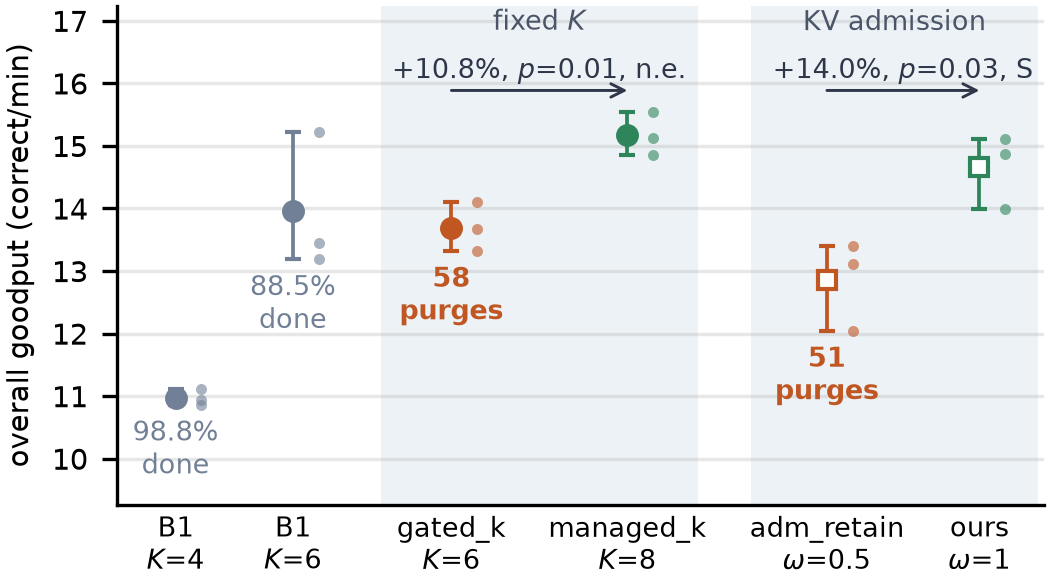
\includegraphics[width=\columnwidth]{../figures/phase2/f2b_dev.png}
  \caption{2\x2 at 16k\,\x4 on dev (mean, min--max, reps). Grey: no gate, orange: llama.cpp
  lifecycle behind the active gate, green: our lifecycle behind the full gate; arrows: lifecycle
  effects (Welch $p$, verdict). 8k\,\x1: Fig.~\ref{fig:2x2_8k}.}
  \label{fig:decomp}
\end{figure}

\subsection{Where the Gain Comes From}\label{sec:decomp}
A 2\x2 at both tight points crosses fixed \K{} with KV admission and llama.cpp's purge with our
lifecycle (Table~\ref{tab:effects}, Fig.~\ref{fig:decomp}). \emph{Gate.} At the same \K, the active
gate completes 99--100\% of tasks where B1 loses up to 36\%, with no significant goodput change;
completing everything lets the 95\% rule choose a higher \K{} (6 instead of 4; 3 instead of 2),
giving +24.8\% and +17.0\%, both S. This is a gain from running more agents safely, not from the
lifecycle, and on test \cfg{gated\_k} is within 4.8\% of \cfg{ours}. \emph{Lifecycle.} Replacing
llama.cpp's purge (51--138 purges per run) with our lifecycle adds 10--16\% in all four comparisons,
but only one is supported. \emph{Admission.} Peak projection never beat a tuned fixed \K{} ($-$2 to
$-$7\%, n.e.), and the best untrimmed dev cell at both points is \cfg{managed\_k} (15.18, 16.68).
\emph{Ablations} (16k\,\x4): removing the drop to the prefix (\cfg{act\_erase}: $-8.7\%$, one run, 4\x{}
the re-prefill) or the host tier (\cfg{ours\_h0}: $-8.4\%$, $p=0.09$) cost the most; always offloading
(\cfg{act\_offload}: +4.3\%, 4 reps, $p=0.31$) and single-run changes of the TTL, the victim order or
delay knowledge ($\pm4.3\%$) are not distinguishable from \cfg{ours}. Which lifecycle parts matter is
therefore not established.

\begin{table}[t]
  \caption{TRIM Selectors at Ample Memory (64k\,\x1, B1 $K{=}8$, 2 Reps)}
  \label{tab:sel}
  \centering
  \scriptsize
  \setlength{\tabcolsep}{2.2pt}
  \begin{tabular}{@{}lrrrrrr@{}}
    \toprule
     & \multicolumn{3}{c}{Perf (selection)} & \multicolumn{3}{c}{Dev (evaluation)} \\
    \cmidrule(lr){2-4}\cmidrule(l){5-7}
    Selector & F1 & Peak ctx & Kept (\%) & F1 & $\Delta$F1 [90\% CI] & KV held \\
    \midrule
    none & 0.588 & 3,140 & 100 / 100 & 0.617 & & 2,248 \\
    oracle & 0.642 & 2,471 & 12 / 100 & 0.670 & [+.022, +.083] & 1,643 \\
    \textbf{relevance:2}\pick & 0.619 & \textbf{2,512} & 17 / 75 & 0.656 & [+.010, +.068] & 1,677 \\
    relevance:3 & 0.626 & 2,519 & 21 / 79 & -- & -- & -- \\
    referenced & 0.609 & 2,664 & 43 / 77 & -- & -- & -- \\
    drop & 0.606 & 2,461 & 7 / 0 & 0.650 & [+.000, +.066] & 1,612 \\
    \bottomrule
  \end{tabular}\\[2pt]
  \parbox{\columnwidth}{\raggedright\scriptsize \pick{} chosen by the pre-registered rule among the
  realistic selectors (\cfg{oracle} and \cfg{drop} are reference points). Peak ctx: per task, the
  largest slot content, mean. Kept: share of observation characters / of supporting-fact sentences.
  KV held: slot tokens when a search or lookup starts, after the compaction (mean).}
\end{table}

\subsection{TRIM Alone}\label{sec:trimalone}
\emph{Quality and KV at ample memory.} No selector lowered F1 (Table~\ref{tab:sel}): on dev,
\cfg{oracle} raised it by 0.053, \cfg{relevance:2} by 0.039 and even \cfg{drop} (titles only) by 0.033,
all with 90\% CIs above 0, and forced finishes fell from 15\% to 10--11\%. The rule chose
\cfg{relevance:2}: within the F1 bound and with the smallest peak context among the realistic
selectors (\cfg{relevance:3} is within 7 tokens). On dev, TRIM cuts the KV held when a tool call
starts by 25--28\% and the per-task peak by 17--19\%. Selectors keeping 7--21\% of the observation text
hold about the same KV, since what remains is mostly the shared prefix and the agent's own Thoughts;
that \cfg{drop} also gains F1 suggests the 7B model is distracted by re-reading paragraphs it has
already summarized. Each compaction prefills about 130 tokens (about 10\% of a task's prefill) and
takes 70--100\,ms (median).

\emph{Fixed concurrency under a tight budget.} TRIM lets B1 run more agents
(Tables~\ref{tab:effects} and~\ref{tab:trim}). At 16k\,\x4 the perf retune moves \K{} from 4 to 6 for
both selectors; on dev, B1 at $K{=}6$ goes from 88.5\% to 100\% completion (+19.9\% with \cfg{oracle},
S), and \cfg{B1+X} beats \cfg{B1}\pick{} by 52.5\% and 45.8\% (both S). This is the best cell measured
at 16k\,\x4, above untrimmed \cfg{ours} by 14.1\% and 9.2\% (n.e.). At 8k\,\x1 \K{} stays 2: TRIM
removes B1's overflows (92\% $\rightarrow$ 100\%) for +12.5\% and +8.0\% (n.e.), and \cfg{B1+X} stays
11--14\% below untrimmed \cfg{ours} (S): even trimmed agents do not fit three at a time.

\begin{table*}[!t]
  \caption{TRIM under the Tight Budgets (Dev, 3 Reps; Untrimmed Rows from Table~\ref{tab:main})}
  \label{tab:trim}
  \centering
  \scriptsize
  \setlength{\tabcolsep}{3.4pt}
  \renewcommand{\arraystretch}{0.9}
  \begin{tabular}{@{}llrrcrrrrrr@{}}
    \toprule
    Point & Config & Knob & Done & Goodput & F1 & Agents & Give-ups & Recomp. & Prefill & Gate wait \\
     & & & (\%) & (correct/min) & & mean (max) & total (off/drop/erase) & (tok/task) & (tok/task) & (s) \\
    \midrule
    16k\,\x4 & \cfg{B1}\pick & $K{=}4$ & 98.8 & 10.97 (10.86--11.11) & 0.621 & 3.9 (4) & -- & 31 & 1,444 & -- \\
     & \cfg{B1}\topk & $K{=}6$ & 88.5 & 13.95 (13.19--15.22) & 0.569 & 5.9 (6) & -- & 187 & 1,626 & -- \\
     & \cfg{ours} & $\omega{=}1$ & 100.0 & 14.66 (13.98--15.11) & 0.635 & 6.8 (10) & 208 (89/118/45) & 472 & 2,221 & 0.20 \\
     & \cfg{B1+oracle} & $K{=}6$ & 100.0 & \textbf{16.73} (16.11--17.20) & 0.658 & 5.9 (6) & -- & 2 & 1,567 & -- \\
     & \cfg{B1+rel2} & $K{=}6$ & 100.0 & 16.00 (15.80--16.10) & 0.640 & 5.9 (6) & -- & 7 & 1,549 & -- \\
     & \cfg{ours+oracle}, no SF & $\omega{=}1$ & 100.0 & 14.14 (13.18--14.69) & 0.662 & 10.1 (13) & 457 (139/318/192) &
      1,548 & 4,341 & 0.71 \\
     & \cfg{ours+rel2}, no SF & $\omega{=}1$ & 100.0 & 13.30 (12.88--13.99) & 0.642 & 9.8 (12) & 445 (136/309/183) &
      1,487 & 4,299 & 0.67 \\
     & \cfg{ours+oracle} & $\omega{=}1$ & 100.0 & 15.58 (15.31--15.83) & 0.658 & 10.1 (13) & 390 (81/309/195) & 1,625 &
      3,892 & 0.48 \\
     & \cfg{ours+rel2} & $\omega{=}1$ & 100.0 & 15.05 (14.32--15.46) & 0.639 & 9.9 (12) & 386 (73/313/193) & 1,639 &
      3,801 & 0.44 \\
    \midrule
    8k\,\x1 & \cfg{B1}\pickf & $K{=}2$ & 92.0 & 12.92 (12.65--13.34) & 0.591 & 2.0 (2) & -- & 8 & 1,398 & -- \\
     & \cfg{ours} & $\omega{=}1$ & 98.8 & \textbf{16.31} (16.09--16.43) & 0.646 & 3.2 (5) & 179 (97/82/57) & 538 & 2,256 &
      0.22 \\
     & \cfg{B1+oracle} & $K{=}2$ & 100.0 & 14.54 (14.27--14.83) & 0.662 & 2.0 (2) & -- & 2 & 1,545 & -- \\
     & \cfg{B1+rel2} & $K{=}2$ & 100.0 & 13.96 (13.37--14.53) & 0.646 & 2.0 (2) & -- & 2 & 1,563 & -- \\
     & \cfg{ours+oracle}, no SF & $\omega{=}1$ & 100.0 & 14.26 (13.51--14.73) & 0.666 & 4.9 (7) & 464 (139/326/231) &
      1,757 & 5,082 & 0.59 \\
     & \cfg{ours+rel2}, no SF & $\omega{=}1$ & 100.0 & 13.29 (12.84--14.18) & 0.649 & 4.8 (6) & 482 (156/326/226) &
      1,736 & 5,146 & 0.59 \\
     & \cfg{ours+oracle} & $\omega{=}1$ & 100.0 & 15.75 (15.58--15.95) & 0.654 & 4.9 (7) & 362 (41/321/236) & 1,969 &
      4,385 & 0.47 \\
     & \cfg{ours+rel2} & $\omega{=}1$ & 100.0 & 15.84 (14.80--16.47) & 0.660 & 4.7 (6) & 356 (50/306/225) & 1,891 &
      4,221 & 0.41 \\
    \bottomrule
  \end{tabular}\\[2pt]
  \parbox{\textwidth}{\raggedright\scriptsize \cfg{B1+X}: B1 at the \K{} its perf retune picked for
  selector X. \cfg{ours+X}: priors refit on trimmed runs, $\omega$ as untrimmed; ``no SF'': without the
  shrink-fast rule (Sec.~\ref{sec:sf}). Agents: time-mean (max: the manager's peak count). Give-ups as in
  Table~\ref{tab:main}. Recomp.: re-prefilled tokens/task, not counting the compactions themselves,
  whose removed text is not lost KV. Prefill: every prompt token the server computed per task. Gate
  wait: mean per request.}
\end{table*}

\subsection{Composing TRIM with the Manager}\label{sec:compose}
\emph{Without shrink-fast}, adding TRIM to \cfg{ours} lost 3.5--18.5\% against untrimmed \cfg{ours}
(S for both selectors at 8k\,\x1). Compaction requests waited behind the gate (0.59--0.71\,s mean
gate wait vs.\ 0.20--0.22\,s untrimmed), and 19--28\% of the manager's eviction operations hit a slot
whose owner had a compaction waiting. Saved before it shrank, such a slot came back as an uncompacted image larger than
the reservation for its shorter prompt (61--99 such restore-bound events per run on average, each
handled by dropping the image and re-prefilling), and the tokens lost at compactions were about twice
the removed text. \emph{With shrink-fast} none of this occurs (0 events), and goodput recovers by
10--19\% (S for \cfg{relevance:2} at 8k\,\x1).

\emph{Admission spends the savings.} Even with shrink-fast, TRIM leaves \cfg{ours} within $-3.4\%$ to
$+6.3\%$ of its untrimmed goodput (all n.e.), although F1 rises by up to 0.02 and TRIM removes the
\texttt{kv\_infeasible} failures at 8k\,\x1. The refit priors (react\_long 0.9-quantile peak 4,904
$\rightarrow$ 3,254--3,276 tokens) let admission run about 50\% more agents (time-mean 10.0 vs.\ 6.8 at
16k\,\x4, 4.8 vs.\ 3.2 at 8k\,\x1). Their idle KV keeps the pool at its cap, so give-ups nearly double
and re-prefilled tokens rise 3.4--3.7\x; total prefill per task is 1.7--1.9\x{} untrimmed \cfg{ours}
and 2.5--2.8\x{} \cfg{B1+X}. With $\omega$ kept at its untrimmed value, TRIM and the lifecycle compete
for the same idle KV instead of adding up: with TRIM, fixed \K{} edges out \cfg{ours} at 16k\,\x4
($-6.8\%$, $-5.9\%$, n.e.), while \cfg{ours} stays ahead at 8k\,\x1 (+8.3\% n.e., +13.5\% S).
Fixed \K{} with our lifecycle plus TRIM (\cfg{managed\_k+X}) and an $\omega$ retune were not run.

\section{Discussion and Limitations}\label{sec:disc}

The measurements answer the project question lever by lever. \emph{Keep it, but count it:} exact
accounting makes committing the pool safe, and running a higher \K{} safely is most of the manager's
gain (+17--25\%, S); 88 full-gate runs (18,800 tasks) had no overflow, no server purge and no failed
restore, and the only reservation breaches were the restore-bound events of the runs without
shrink-fast. \emph{Move it or throw it away:} giving idle KV up per agent adds a consistent 10--16\%
over llama.cpp's purge, and llama.cpp's own host-RAM cache trails the manager by 11--34\%; the
ablations point to the prefix and the host tier rather than to when or whom to evict, though neither
loss is established. \emph{Keep only part of it:} most of
an agent's tool output is dead weight once read; dropping it cuts tool-wait KV by a quarter and
improves answers, which is worth +46--53\% where trimmed agents fit a higher \K{} (16k\,\x4) and +8--13\%
(n.e.) where they do not (8k\,\x1). \emph{Together:} the levers draw on the same slack, so a policy that
turns freed memory into more agents (here, admission with refit priors) moves the cost into
recompute. In practice: with a hand-set concurrency, trim and retune \K; when even trimmed agents fit
too few at a time, use the gate and lifecycle (\cfg{managed\_k} was the best untrimmed configuration;
admission is not needed).

\emph{Limitations.} Protocol: with 2--3 reps, $p$ is indicative, and several comparisons have
$p<0.05$ but a CI including 0. Some reps were added after $n=2$ results were seen (16k\,\x4 and
32k\,\x4 dev; the \cfg{act\_offload} and \cfg{always\_off} ablations), so those $p$-values are
optimistic, and overall goodput became the primary test possibly after dev results were seen
(unrecorded). B1's knobs rest on one perf run per \K. TRIM ran on dev only; the shrink-fast rule is post
hoc; B1's \K{} was retuned under TRIM while $\omega$ was not, and \cfg{managed\_k+X} was not run, so
the composition result holds for admission as tuned without TRIM. Scope: one model and GPU, an offline
corpus easier than full Wikipedia, simulated tool delays, task-specific selectors (\cfg{oracle} uses
labels, \cfg{relevance:2} the question's words), and an iso-memory comparison only for
\cfg{ours\_h0}. Outputs are not deterministic under concurrent CUDA batches, so quality is compared
paired and over reps, never from single runs.

\onecolumn
\appendix[Timeline, Tuning Data and Notes]
\vspace{4pt}

\begin{center}
  \small
  \setlength{\tabcolsep}{5pt}
  \begin{tabular}{@{}L{0.11\textwidth}L{0.55\textwidth}L{0.22\textwidth}L{0.06\textwidth}@{}}
    \toprule
    Dates & Work & Milestone & Status \\
    \midrule
    10/21--10/28 & Design; data, corpus, splits; tools, ReAct agent, profiles; workload generator; FIFO
      runner and instrumentation & End-to-end workload on 7B & Done \\
    10/29--11/4 & AWS A10G setup; cost model; runtime probes; microbenchmarks; workload and
      bottleneck measurements; Phase 1 report & \textbf{Phase 1 due 11/4} & Done \\
    11/5--11/15 & Slot-control probes; KV manager: exact ledger and gate, peak-projection admission,
      offload/drop/erase lifecycle with online cost model; cell-level llama-server mock & Manager runs
      end to end with zero violations & Done \\
    11/15--11/16 & Baseline and $\omega$ tuning on perf; active-gate fix; dev comparison at four points;
      2\x2 at 16k\,\x4; ablations & Phase 2 results & Done \\
    11/17--11/18 & Third reps at 8k\,\x1 and 16k\,\x1; 2\x2 at 8k\,\x1; held-out test split &
      Claims tested on held-out data & Done \\
    11/17--11/18 & TRIM: eager compaction, selectors, offline replay; selector choice and quality;
      B1 retune; dev runs with B1 and the manager; shrink-fast rule and rerun & Phase 3 results & Done \\
    11/19--12/9 & Final report, technical notes and reproducibility package &
      \textbf{Final submission 12/9} & In progress \\
    \bottomrule
  \end{tabular}
\end{center}

\begin{figure}[h]
  \centering
  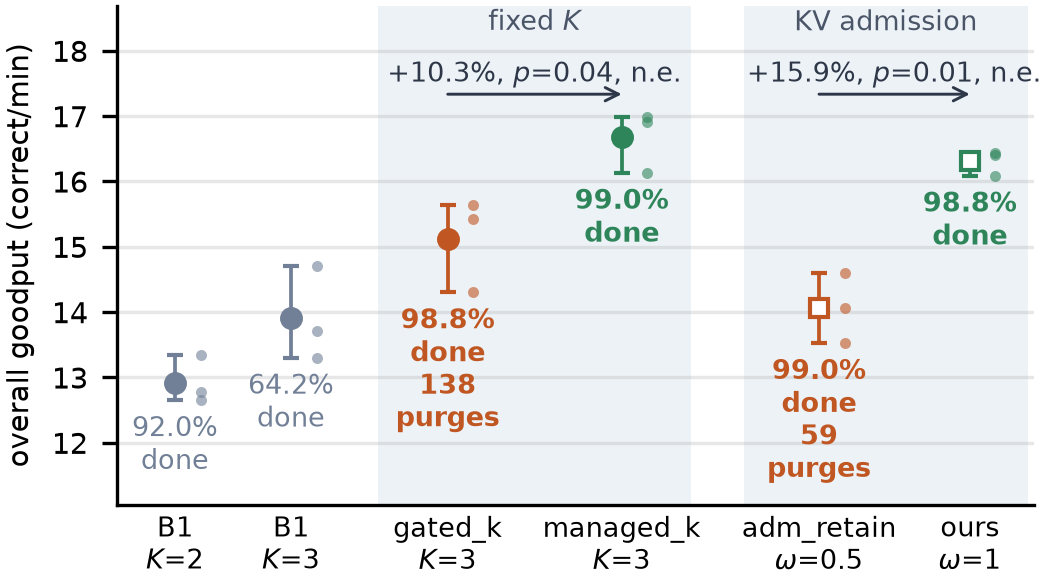
\includegraphics[width=3.5in]{../figures/phase2/f2c_dev_8k.png}
  \caption{2\x2 at 8k\,\x1 on dev, drawn as Fig.~\ref{fig:decomp} (\cfg{gated\_k} and
  \cfg{managed\_k} at $K{=}3$, \cfg{adm\_retain} at $\omega{=}0.5$). Bold \%: completion below 99.5\%.}
  \label{fig:2x2_8k}
\end{figure}

\begin{figure}[h]
  \centering
  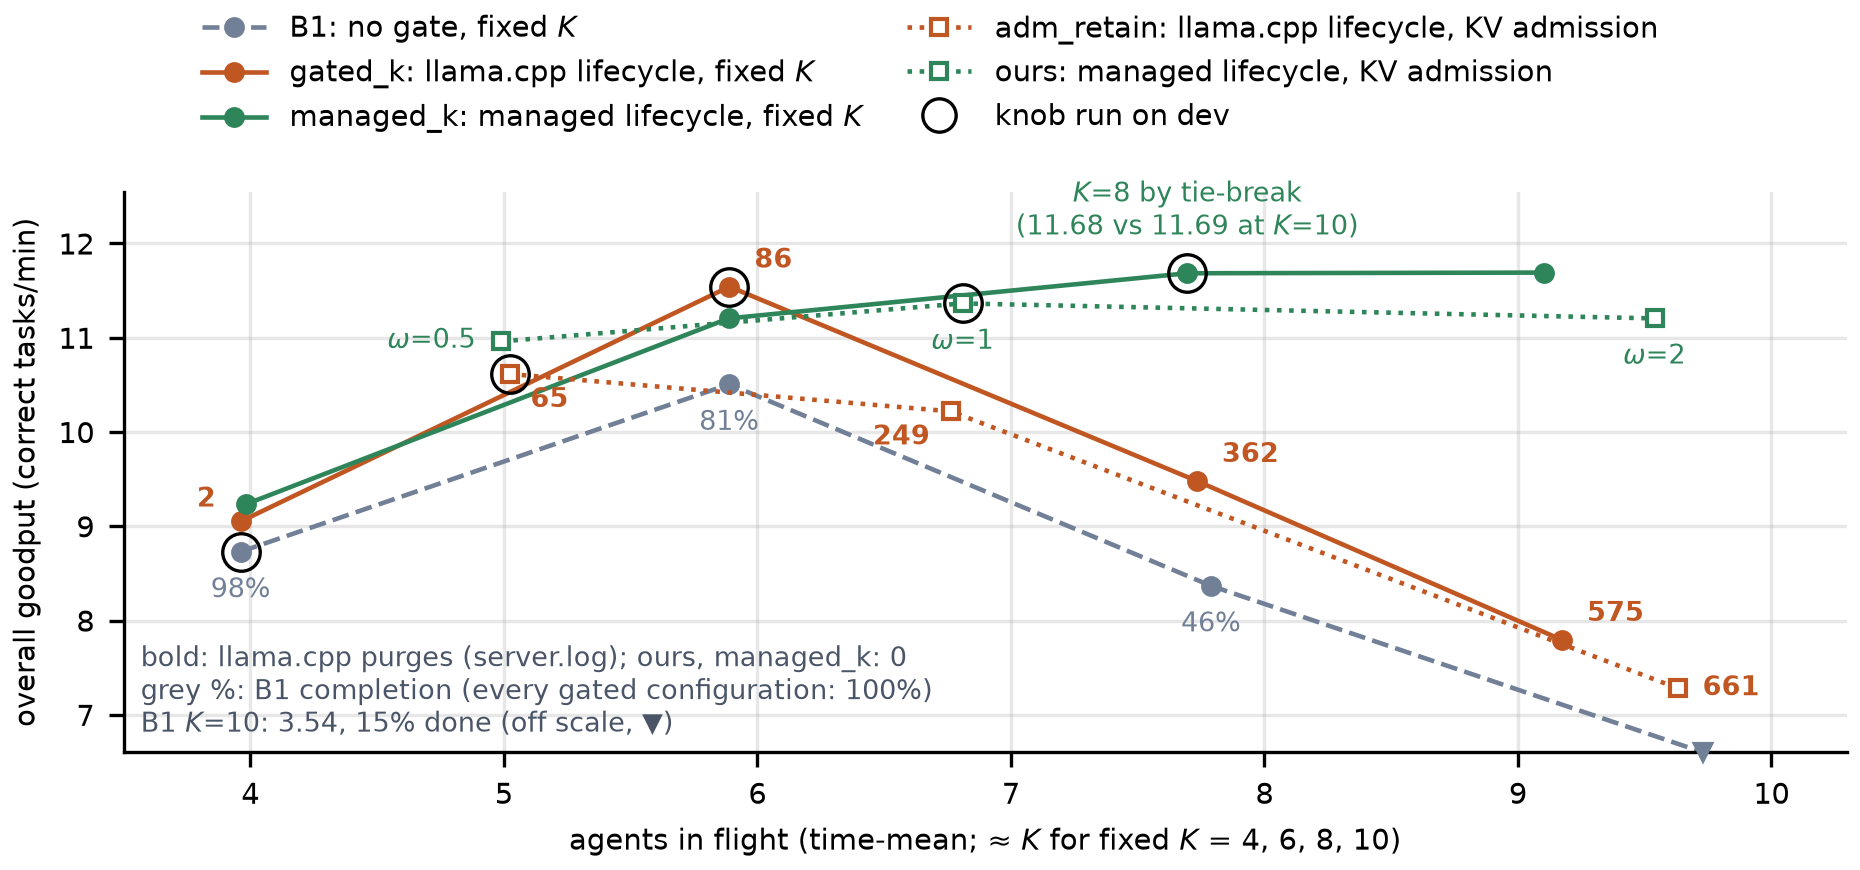
\includegraphics[width=6.2in]{../figures/phase2/f2a_tuning.png}
  \caption{Perf tuning runs at 16k\,\x4, one per knob (selection data, not results). Circles = knob
  run on dev in Fig.~\ref{fig:decomp} (\cfg{managed\_k}: $K{=}8$ by a tie-break fixed before the dev
  runs; the goodput rule gives $K{=}10$); bold = llama.cpp purges per run; grey \% = B1 completion.}
  \label{fig:tuning}
\end{figure}

\medskip
\noindent\emph{Tuning without TRIM} is shown in Fig.~\ref{fig:tuning} for 16k\,\x4: the active gate
peaks at $K{=}6$ and falls as purges rise, while our lifecycle holds its goodput from $K{=}6$ to 10.

\medskip
\noindent\emph{B1 retuned under TRIM} (perf, one run per \K; goodput / completion). 16k\,\x4,
\cfg{oracle}: $K{=}4$ 10.14 / 100\%, $\mathbf{K{=}6}$ 13.68 / 97\%, $K{=}8$ 16.25 / 81.5\%, $K{=}10$
3.44 / 16\%; \cfg{relevance:2}: 10.53 / 100\%, $\mathbf{15.27}$ / 97\%, 15.79 / 88.5\%, 6.17 / 21.5\%.
8k\,\x1, \cfg{oracle}: $\mathbf{K{=}2}$ 13.17 / 100\%, $K{=}3$ 16.90 / 91\%, $K{=}4$ 10.16 / 30.5\%,
$K{=}5$ 1.39 / 3.5\%; \cfg{relevance:2}: $\mathbf{13.10}$ / 100\%, 15.98 / 86.5\%, 8.16 / 31\%, 1.06 /
3\%. Without TRIM, the same rule picked $K{=}4$ (8.73 / 98\%) and $K{=}2$ (10.24 / 89\%, fallback). Each
grid has one \K{} more than the untrimmed grid, added before any run.

\medskip
\noindent\emph{Active-gate bug.} In tuning, two of three \cfg{adm\_retain} runs overflowed: the
active gate charged a reused slot at $f$ instead of $\max(s,f)$. All three pre-fix runs were
excluded and the cell re-tuned. Only the two active-gate configurations use this gate; the full-gate
configurations and all dev and test runs are unaffected.

\medskip
\noindent\emph{Shrink-fast test.} The rule (\texttt{KVConfig.shrink\_fast}) is tested on the
cell-level llama-server mock: four agents in a pool that fits about three, every compaction dispatched
at once and none of their slots evicted while waiting. With the flag off, the runs without shrink-fast
are reproduced.

\medskip
\noindent\emph{Artifacts.} Code, configs and generators: \texttt{edgeserve/} (agent, runner, manager,
TRIM), \texttt{configs/sweeps/}, \texttt{analysis/phase2\_report.py} and
\texttt{analysis/phase3\_report.py} (every table, from \texttt{results/runs.csv}), technical notes
in \texttt{docs/}.

\begin{thebibliography}{9}
\footnotesize
\bibitem{llamacpp} G.~Gerganov \emph{et al.}, ``llama.cpp,'' \url{https://github.com/ggml-org/llama.cpp}.
\bibitem{qwen} Qwen Team, ``Qwen2.5 technical report,'' arXiv:2412.15115, 2024.
\bibitem{hotpotqa} Z.~Yang \emph{et al.}, ``HotpotQA: A dataset for diverse, explainable multi-hop question
answering,'' in \emph{Proc. EMNLP}, 2018.
\bibitem{react} S.~Yao \emph{et al.}, ``ReAct: Synergizing reasoning and acting in language models,'' in
\emph{Proc. ICLR}, 2023.
\bibitem{vllm} W.~Kwon \emph{et al.}, ``Efficient memory management for large language model serving with
PagedAttention,'' in \emph{Proc. SOSP}, 2023.
\bibitem{sglang} L.~Zheng \emph{et al.}, ``SGLang: Efficient execution of structured language model
programs,'' in \emph{Proc. NeurIPS}, 2024.
\bibitem{infercept} R.~Abhyankar \emph{et al.}, ``InferCept: Efficient intercept support for augmented
large language model inference,'' in \emph{Proc. ICML}, 2024.
\bibitem{llmlingua} H.~Jiang \emph{et al.}, ``LLMLingua: Compressing prompts for accelerated inference of
large language models,'' in \emph{Proc. EMNLP}, 2023.
\bibitem{h2o} Z.~Zhang \emph{et al.}, ``H$_2$O: Heavy-hitter oracle for efficient generative inference of
large language models,'' in \emph{Proc. NeurIPS}, 2023.
\end{thebibliography}

\end{document}
